\setcounter{page}{1}
\section*{Zielsetzung}
In diesem Versuch sollen die Grundlagen der Rastertunnelmikroskopie
erlernt werden.
Hierzu wird die Oberfläche einer HOPG-Struktur (Graphit) und einer
Goldprobe untersucht. Mit Hilfe der Oberflächenmessung sollen die Gittervektoren
einer HOPG-Struktur bestimmt werden und das Höhenprofil einer Goldprobe untersucht werden.

\section{Theorie}
Die Funktionsweise eines Rastertunnelmikroskops (RTM) beruht auf dem, aus der Quantenmechanik bekannten, %dem
\emph{Tunneleffekt}. Dieser erlaubt es Elektronen in klassisch verbotene Bereiche zu \emph{tunneln}. %Elektronen
Beim Tunneln durchqueren die Elektronen ein Potential, welches sie im klassischen Sinne
eigentlich nicht überwinden können (vgl. Abb. \ref{fig: tunneleffekt}).
\begin{figure}[!h]
  \centering
  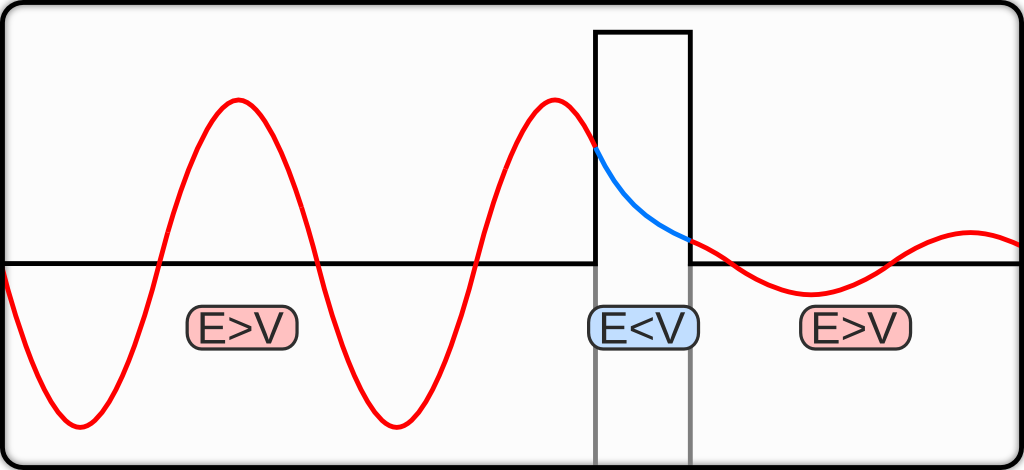
\includegraphics[width=0.6\textwidth]{./pics/tunelleffekt.png}
  \caption{Darstellung des Tunneleffekts.
  Das Elektron durchquert ein Potential $V$, obwohl seine Energie $E$ dafür eigentlich nicht ausreicht. \cite{tunnel}}
  \label{fig: tunneleffekt}
\end{figure}
Der Tunneleffekt spielt zum Beispiel beim $\alpha$-Zerfall eine zentrale Rolle, hier tunnelt ein Heliumkern durch das Coulombpotential. %leerzeichen
Das Rastertunnelmikroskop bietet die Möglichkeiten bis in den atomaren Bereich genau aufzulösen\cite{aufl}. %denke noch genauer

Der Tunneleffekt wird bei einem RTM verwendet, um einen \emph{Tunnelstrom} zu erzeugen. Dieser Tunnelstrom
fließt zwischen der Messspitze des Mikroskops und der Probe.
Der gemessene Tunnelstrom ist proportional zu %Absatz
\begin{equation}
  \label{eq: tunnelstrom}
I\propto \frac{U}{d}\exp{(-kd\sqrt{\phi}) }.
\end{equation}
Dabei ist $d$ der Abstand zwischen Spitze und Probe, $U$ die zwischen Spitze und Probe anliegende Spannung,
$\phi$ die durchschnittliche Elektronaustrittsarbeit zwischen Spitze und Probe und $k$ eine Konstante, die im Vakuum gegeben ist als
\begin{equation*}
  k=\SI{1.025}{\per\angstrom\sqrt{\eV}}.
\end{equation*}
Mit Hilfe der Rastertunnelmikroskopie werden Proben so detailreich aufgelöst, dass thermische Effekte eine Rolle spielen. %kein werden nach detailreich
So haben durch Temperaturänderung verursachte thermische Drifts, eine signifikante Auswirkung auf die Messung. %satz überarbeiten%Abschnitt nochmal überarbeiten
Eine Temperaturänderung wird zum Beispiel durch das Anfassen der Probe verursacht.
Damit die durch die thermischen Effekte verursachten Fehlern verkleinert werden,
werden die Richtungen der Oberflächenmessung unterschieden.

\subsection{Piezokeramiken}

Die hohen Genauigkeiten eines Rastertunnelmikroskops werden durch Ausnutzung des
\emph{piezoelekttrischen Effekts} erreicht. %Hier noch erwähnen, dass die Ausdehnung zur mechanischen Bewegung der Spitze genutzt werden
Stoffe, die dem piezoelektrischen Effekt unterliegen werden als Piezokristall %doppelt Effekt
oder als Piezokeramik (vgl. Abb. \ref{fig: piezo}) bezeichnet.
\begin{figure}[!h]
  \centering
  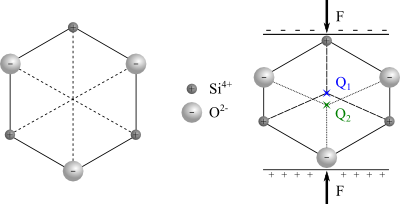
\includegraphics[width=0.6\textwidth]{./pics/piezo.png}
  \caption{Schemtischer Aufbau eines Piezokristalls (links). Außerdem ist die Änderung der räumlichen Struktur, auf Grund eines
  äußeren Elektrischenfeldes, zu erkennen (rechts). \cite{piezo}.}
  \label{fig: piezo}
\end{figure}
Ein Piezokristall besitzt die Eigenschaft, sich unter Einwirkung eines äußeren
elektrischen Feldes auszudehnen bzw. zusammenzuziehen.
Dabei findet die Ausdehnung immer parallel zur
Ausrichtung des elektrischen Feldes statt und ist mit den in dem Kristall wirkenden
Dipolmomenten zu erklären. In erster Näherung ist die Ausdehnung linear mit der anliegenden Feldstärke,
jedoch ist in Wirklichkeit ein nicht linearer Zusammenhang zwischen Ausdehnung und Feldstärke
gegeben (vgl. Abb. \ref{fig: non_linear}). Diese Nichtlinearität sorgt dafür, dass die Qualität der aufgenommenen Bilder
vermindert wird. Die Ausdehnung des Kristalls wird dazu verwendet, um die Spitze des Rastertunnelmikroskops zu manövrieren.
\begin{figure}[!h]
  \centering
  \includegraphics[width=0.6\textwidth]{./pics/nicht_linearität.png}
  \caption{Schematische Darstellung der Nichtlineraität der Ausdehnung eines Piezokristalls \cite{rtm}.} %Ausdehnung
  \label{fig: non_linear}
\end{figure}

Neben der Nichtlinearitiät der Ausdehnung verschlechtern noch weitere %linearität
Effekte die Genauigkeit eines RTM. Hierzu gehören zum Beispiel Hystereseeffekte (vgl. Abb. \ref{fig: hysterese}) die dafür sorgen,
dass Messungen richtungsabhängig sind.
\begin{figure}[!h]
  \centering
  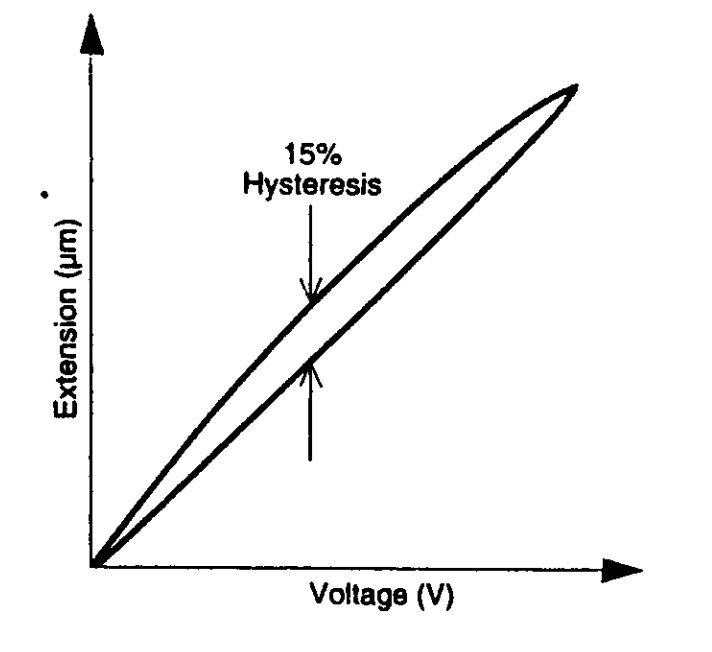
\includegraphics[width=0.6\textwidth]{./pics/hysterese.png}
  \caption{Schematische Darstellung der Hysterese einer Piezokeramik \cite{rtm}.}
  \label{fig: hysterese}
\end{figure}
Bei einer abrupten Spannungsänderung ändert der Kristall seine Auslenkung nicht instantan, sondern benötigt erst eine gewisse Zeit.
Dieser Effekt, der als \emph{Kriechen} bezeichnet wird, kann bis zu $\SI{100}{\second}$ andauern.
Durch das Kriechen sehen eigentlich eckige Strukturen gekrümmt aus (vgl. Abb. \ref{fig: creep}).
\begin{figure}[!h]
  \centering
  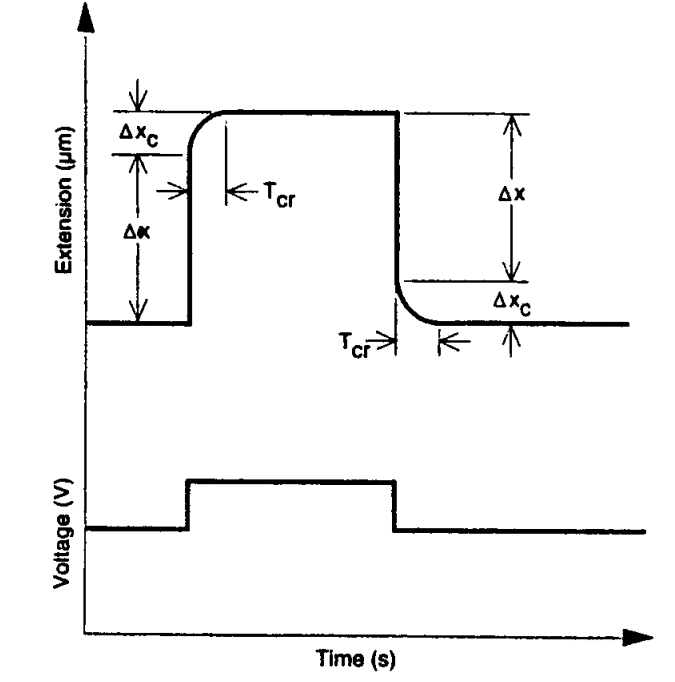
\includegraphics[width=0.6\textwidth]{./pics/creep.png}
  \caption{Auswirkung des Kriechens auf eine Messung mit einem RTM \cite{rtm}.}
  \label{fig: creep}
\end{figure}
Außerdem unterliegt eine Piezokeramik einem Effekt, der als \emph{Alterung} bezeichnet wird. Der Effekt besagt,
dass bei langer nicht Verwendung des Kristalls sich die Ausdehnungsfähigkeit verringert. Erklärbar ist der Effekt mit den %dass, verb fehlt
Dipolmomenten im Kristall, die Momente richten sich bei langer Nichtbenutzung willkürlich aus und verringern %wenn dann Nichtbenutzung oder anderes Wort
somit die Empfindlichkeit auf äußere Feldänderungen (vgl. Abb. \ref{fig: ageing}).
\begin{figure}[!h]
  \centering
  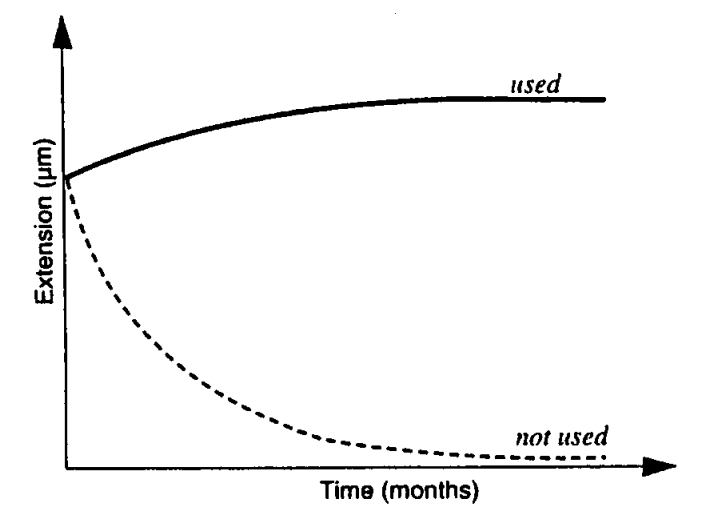
\includegraphics[width=0.6\textwidth]{./pics/ageing.png}
  \caption{Schematische Darstellung des Verhaltens eines Piezokristalls bei häufiger und weniger Benutzung \cite{rtm}.} %Schematische Darstellung, kristalls, häufiger
  \label{fig: ageing}
\end{figure}
Es ist möglich nach einer Zeit der Nichtverwendung
durch häufiges Benutzen die Empfindlichkeit wieder zu verbessern.
Das Phänomen der \emph{Kreuzkopplung} beschreibt die $x$- und $y$-Abhängigkeit der $z$-Komponente des Piezokristalls (vgl. Abb. \ref{fig: cross_copeling}). %kristalls
Die damit verbundenen Fehler können mit Hilfe einer Software rausgerechnet werden. %Satz vielleicht noch vor der Abbildung
\begin{figure}[!h]
  \centering
  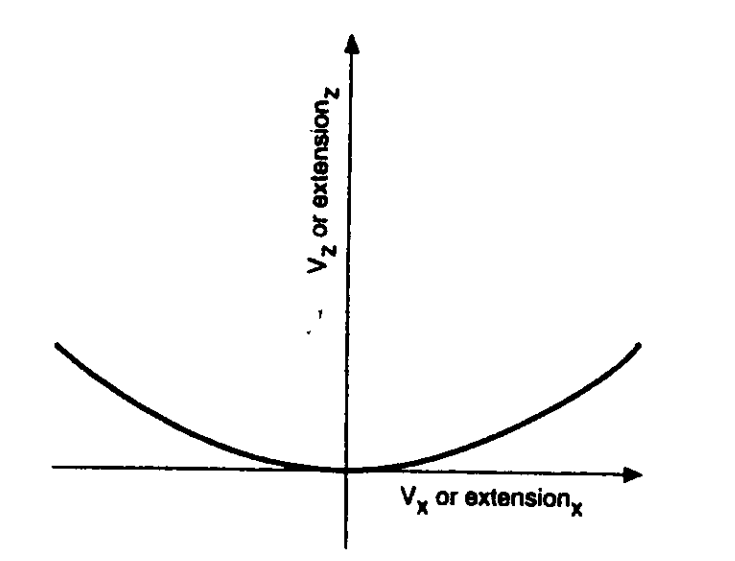
\includegraphics[width=0.6\textwidth]{./pics/cross_copling.png}
  \caption{Schmeatische Darstelung der Auslenkung der Kreuzkopplung \cite{rtm}.}
  \label{fig: cross_copeling}
\end{figure}

%thermische Drifts
\subsection{HOPG}
HOPG (Highly oriented pyrolytic graphite) ist ein Graphit, welches sich durch einen besonders hohen Grad
an Ordnung auszeichnet. Deshalb wird diese Graphitstruktur oftmals verwendet, um sich ein Rastertunnelmikroskop zu kalibrieren und
um sich mit dem Gerät vertraut zu machen. %und zur Kallibrierung
Die atomare Struktur von HOPG %nur die schichten, atome untereinander über kovalente Bindung (nicht sicher, nochmal nachlesen) (hier)s
ist in Abbildung \ref{fig: hopg} illustriert.
\begin{figure}[!h]
  \centering
  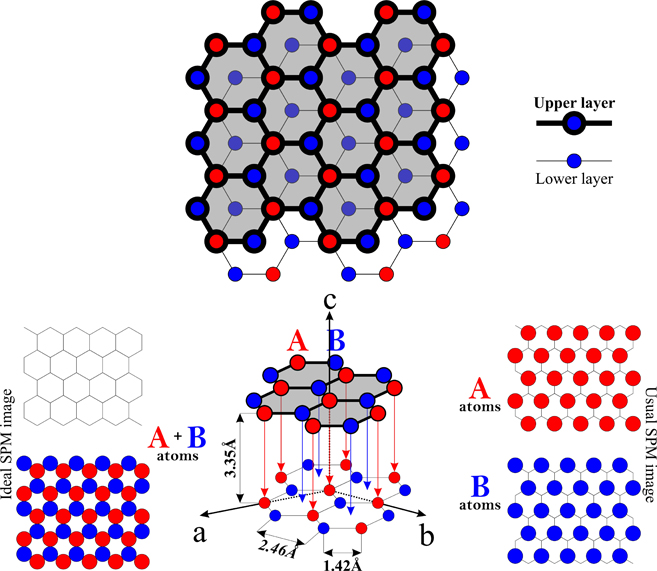
\includegraphics[width=0.6\textwidth]{./pics/hopg.jpg}
  \caption{Atomarer Aufbau von HOPG \cite{hopg}.}
  \label{fig: hopg}
\end{figure}
Wie in der Abbildung zu erkennen ist, sind die Atome hexagonal angeordnet. Außerdem besitzen sie einen Abstand von ca.
$\SI{1.45}{\angstrom}$ \cite{hopg}. %Vielleicht besser den für uns relevanten ABstand aufführen (hier)
